%DIF PREAMBLE EXTENSION ADDED BY LATEXDIFF
%DIF UNDERLINE PREAMBLE %DIF PREAMBLE
\RequirePackage[normalem]{ulem} %DIF PREAMBLE
\RequirePackage{color}\definecolor{RED}{rgb}{1,0,0}\definecolor{BLUE}{rgb}{0,0,1} %DIF PREAMBLE
\providecommand{\DIFadd}[1]{{\protect\color{blue}\uwave{#1}}} %DIF PREAMBLE
\providecommand{\DIFdel}[1]{{\protect\color{red}\sout{#1}}}                      %DIF PREAMBLE
%DIF SAFE PREAMBLE %DIF PREAMBLE
\providecommand{\DIFaddbegin}{} %DIF PREAMBLE
\providecommand{\DIFaddend}{} %DIF PREAMBLE
\providecommand{\DIFdelbegin}{} %DIF PREAMBLE
\providecommand{\DIFdelend}{} %DIF PREAMBLE
%DIF FLOATSAFE PREAMBLE %DIF PREAMBLE
\providecommand{\DIFaddFL}[1]{\DIFadd{#1}} %DIF PREAMBLE
\providecommand{\DIFdelFL}[1]{\DIFdel{#1}} %DIF PREAMBLE
\providecommand{\DIFaddbeginFL}{} %DIF PREAMBLE
\providecommand{\DIFaddendFL}{} %DIF PREAMBLE
\providecommand{\DIFdelbeginFL}{} %DIF PREAMBLE
\providecommand{\DIFdelendFL}{} %DIF PREAMBLE
%DIF END PREAMBLE EXTENSION ADDED BY LATEXDIFF

%\documentclass{sigplanconf}
%\nocaptionrule

% \documentclass[twocolumn,9pt]{article}
% \documentclass[twocolumn,10pt]{acm_proc_article-sp}

% \documentclass{acm_proc_article-sp}
\documentclass[9pt]{sigplanconf}

\date{} % \vspace*{-0.2in}}

% Make sure to put back 

\newcommand{\punt}[1]{}

\punt{

Notes from Daan Leijen:
}

\usepackage{endnotes,xspace}

\newcommand{\footnotenonumber}[1]{{\def\thempfn{}\footnotetext{\small #1}}}
\usepackage[normalem]{ulem}
\usepackage{graphicx}

\usepackage{mathptmx} % rm & math
\usepackage[scaled=0.90]{helvet} % ss
\usepackage{courier} % tt
% \normalfont
\usepackage[T1]{fontenc}

% \usepackage{lmodern}
% \usepackage{times}
\usepackage{subfigure}
\usepackage{url}
\urlstyle{rm}
\usepackage[
      colorlinks=false,    %no frame around URL
      urlcolor=black,    %no colors
      menucolor=black,    %no colors
      linkcolor=black,    %no colors
      pagecolor=black,    %no colors
]{hyperref}

\usepackage{color}
\usepackage{listings}
\usepackage{amsmath}
\usepackage{amsfonts}
\usepackage{amssymb}
\usepackage{comment} 
\usepackage{setspace}
\singlespacing
%\onehalfspacing
\newtheorem{thm}{Theorem}
\newtheorem{prop}[thm]{Proposition}
\newtheorem{cor}[thm]{Corollary}
\newtheorem{lem}[thm]{Lemma}
\newtheorem{defn}[thm]{Definition}

\newcommand{\cfunction}[1]{{\bf \tt #1}}
\newcommand{\malloc}{\cfunction{malloc}}
\newcommand{\realloc}{\cfunction{realloc}}
\newcommand{\free}{\cfunction{free}}
\newcommand{\madvise}{\cfunction{madvise}}
\newcommand{\brk}{\cfunction{brk}}
\newcommand{\sbrk}{\cfunction{sbrk}}
\newcommand{\mmap}{\cfunction{mmap}}
\newcommand{\munmap}{\cfunction{munmap}}
\newcommand{\mprotect}{\cfunction{mprotect}}
\newcommand{\mlock}{\cfunction{mlock}}

\hyphenation{app-li-ca-tion}
\hyphenation{Die-Hard}
\hyphenation{Ar-chi-pe-la-go}
\hyphenation{buf-fer}
\hyphenation{D-threads}
\hyphenation{Heap-Layers}
\hyphenation{wait-Token}
\hyphenation{mul-ti-threa-ded}
\hyphenation{me-m-ory}

\hyphenation{pthread-create}
\hyphenation{pthread-self}
\hyphenation{pthread-mutex-lock}
\hyphenation{pthread-mutex-unlock}

\newcommand{\dthreads}{{\scshape Dthreads}}
\newcommand{\Dthreads}{{\scshape Dthreads}}
\newcommand{\doubletake}{{\scshape DoubleTake}}
\newcommand{\DoubleTake}{{\scshape DoubleTake}}
\newcommand{\stopgap}{{\scshape DoubleTake}}
\newcommand{\Stopgap}{{\scshape DoubleTake}}
\newcommand{\StopGap}{{\scshape DoubleTake}}
\newcommand{\Sheriff}{{\scshape Sheriff}}
\newcommand{\sheriff}{{\scshape Sheriff}}
\newcommand{\Grace}{{\scshape Grace}}
\newcommand{\grace}{{\scshape Grace}}
\newcommand{\SheriffProtect}{\textsc{Sheriff-Protect}}
\newcommand{\sheriffProtect}{\textsc{Sheriff-Protect}}
\newcommand{\sheriffprotect}{\textsc{Sheriff-Protect}}
\newcommand{\SheriffDetect}{\textsc{Sheriff-Detect}}
\newcommand{\sheriffDetect}{\textsc{Sheriff-Detect}}
\newcommand{\sheriffdetect}{\textsc{Sheriff-Detect}}
\newcommand{\pthreads}{\texttt{pthreads}}

\definecolor{lightgray}{rgb}{.9,.9,.9}
\definecolor{darkgray}{rgb}{.4,.4,.4}
\definecolor{purple}{rgb}{0.65, 0.12, 0.82}

\lstdefinelanguage{c++threads}[]{c++}{
  morekeywords={pthread_create,pthread_join},
  keywordstyle=\color{blue}\bfseries,
  ndkeywords={class, export, boolean, throw, implements, import, this},
  ndkeywordstyle=\color{darkgray}\bfseries,
  identifierstyle=\color{black},
  sensitive=false,
  comment=[l]{//},
  morecomment=[s]{/*}{*/},
  commentstyle=\color{purple}\ttfamily,
  stringstyle=\color{red}\ttfamily,
  morestring=[b]',
  morestring=[b]"
}
\lstset{
   language=c++threads,
   backgroundcolor=\color{lightgray},
   extendedchars=true,
   basicstyle=\footnotesize\ttfamily,
   showstringspaces=false,
   showspaces=false,
   numbers=none,
   numberstyle=\footnotesize,
   numbersep=9pt,
   tabsize=2,
   breaklines=true,
   showtabs=false,
   captionpos=b
}
%\lstset{language=c++threads, basicstyle=\ttfamily\scriptsize,frame=trbl,tabsize=4} % ,numbers=left,numberstyle=\tiny}

\definecolor{Gray}{cmyk}{0,0,0,0.5}

\begin{document}

\CopyrightYear{2014}
\copyrightdata{XXX-X-XXXXX-XXX-X/XX/XX}

\title{{\huge \bf \doubletake{}}: Evidence-Based Dynamic Analysis}
% Efficiently and Precisely Locating Buffer Overflows}

% \authorinfo{\emph{authorship list removed for anonymity}}

%\punt{
\authorinfo{Tongping~Liu \and Charlie~Curtsinger \and Emery~D.~Berger}
{School of Computer Science \\
University of Massachusetts Amherst \\
Amherst, MA 01003 \\
{\{tonyliu,charlie,emery\}@cs.umass.edu}
}

\punt{
\numberofauthors{1}
\author{
\alignauthor Tongping~Liu and Emery~D.~Berger \\
\affaddr{Department of Computer Science} \\
\affaddr{University of Massachusetts, Amherst} \\
\affaddr{Amherst, MA 01003} \\
\email{\{tonyliu,emery\}@cs.umass.edu} \\
}
}

\maketitle

\begin{comment}
\end{comment}

\begin{abstract}
%How is existing work?
%Sharing inside mulithreaading programs is not easy, they can easily cause correctness or performance problem. 
%Inappropriate sharing can dramatically degrade the performance of 
%mulithreading programs and seriously affect the scalability. 
%So detecting false sharing accurately and precisely can be helpful for user to fix corresponding performance problem. 

\begin{comment}
False sharing is notorious for performance degradation in multithreaded
programs. It apprears when two or more threads running on different cores periodically access 
different portions of data that can fit into one cache line. Since caching
system in a multicore processor needs to ensure a coherent view of memory
accross all cores, it has to grant an exclusive access
for each write operation by invidating duplicate copies in other cores. As a
result, frequent cache invalidation can seriously affect the scalability and
performance of multithreaded programs.
\end{comment} 

False sharing is a notorious performance issue for different software stacks, 
which can dramatically degrade the performance and seriously affect the scalability of 
systems.

%Many reserach efforts have been made to detect false sharing. 
Unfortunately, previous approaches to detect false sharing
either introduce significant performance overhead, or fail
to report false sharing accurately and precisely, or have different limitations of usage. 
%\sheriff{}, the prior state-of-the-art tool, 
%can only detect write-write false sharing in applications using \pthreads{} library.
This paper presents a novel approach, \Predator{}, to combine compiler instrumentation
and runtime system to detect false sharing. 
%the compiler instruments every memory access and 
%the runtime system collects and analyzes memory accesses to detect false sharing problems.
Since it does not rely on any hardware, OS or threading library, this approach can be
applied to the entire software stack without any limitation. 
\Predator{} can detect false sharing accurately and precisely: it reports no 
false positives and pinpoints exact objects with false sharing problems.
%Also, unlike previous work, this method can be extended to
%identify false sharing problems across the entire software stack, including 
%hypervisors, operating systems, libraries and applications. 
Experimental results on two popular benchmark suites 
show that \Predator{} not only detected all known false sharing problems but also revealed 
two unknown false sharing problems.
Besides, \Predator{} have successfully detected false sharing of real applications,
including \texttt{mysql} server application and \texttt{boost} library. Fixing these
false sharing problems improves performance by $6\times$ and $40\%$ correspondingly.

Moreover, existing tools can only detect those manifested false sharing problems.
However, occurrences of false sharing can be affected by alignments between
objects and cache lines: any change of compiler optimization, compiler, memory manager, 
memory allocation order, cache line size or different target binary 
may change alignments, and thus affect occurrences of false sharing, 
which leaves many of them undetected by existing tools.
\Predator{} is the first tool which can accurately predict possible false sharing 
without the need of occurrences. 
It can report all false sharing problems with only one execution and with reasonable overhead, 
around $6.7\times$ performance overhead on average.

%What is novel in our work?
%How is the performance overhead?


\end{abstract}

%  Language-based approaches require programmers to write their code in specialized languages. 


\punt{
\category{D.1.3}{Programming Techniques}{Concurrent Programming--Parallel Programming}
\category{D.2.5}{Software Engineering}{Testing and Debugging--Debugging Aids}

\terms
Design, Reliability, Performance

\keywords
Buffer Overflow, Detection 
}


%%%%%%%%%%%%%%%%%%%%%%%%%%%%%%%%%%%%%%%%%%%%%%%%%%%%%%%%%%%%%%%%%%%%%%%%%%%%%%%%%%%%%%%%%%%%%
%%%%%%%%%%%%%%%%%%%%%%%%%%%%%%%%%%%%%%%%%%%%%%%%%%%%%%%%%%%%%%%%%%%%%%%%%%%%%%%%%%%%%%%%%%%%%

\section{Introduction}
\label{sec:introduction}

The advent of multicore architectures has increased the demand for multithreaded
programs, but writing them remains painful. It is notoriously far more
challenging to write concurrent programs than sequential ones because of the
wide range of concurrency errors, including deadlocks and race
conditions~\cite{havender,76897,130623}. Because thread interleavings are
non-deterministic, different runs of the same multithreaded program can
unexpectedly produce different results. These ``Heisenbugs'' greatly complicate
debugging, and eliminating them requires extensive testing to account for
possible thread
interleavings~\cite{DBLP:conf/icse/BallBHMQ09,DBLP:conf/asplos/BurckhardtKMN10}.

% Lots of recent work on bug finding. Getting better, but still difficult.

Instead of testing, one promising alternative approach is to attack the problem
of concurrency bugs by eliminating its source: non-determinism. A fully
\emph{deterministic multithreaded system} would prevent Heisenbugs by ensuring
that executions of the same program with the same inputs always yield the same
results, even in the face of race conditions in the code. Such a system would
not only dramatically simplify debugging of concurrent
programs~\cite{Carver:1991:RTC:624586.625040} and reduce testing overhead, but
would also enable a number of other applications. For example, a deterministic
multithreaded system would greatly simplify record and replay for multithreaded
programs by eliminating the need to track memory
operations~\cite{Choi:1998:DRJ:281035.281041,LeBlanc:1987:DPP:32387.32396}, and
it would enable the execution of multiple replicas of multithreaded applications
for fault
tolerance~\cite{deterministic-process-groups,1134000,224058,replicant-hotos}.

Several recent software-only proposals aim at providing deterministic
multithreading for C/C++ programs, but these suffer from a variety of
disadvantages. Kendo ensures determinism of synchronization operations with low
overhead, but does not guarantee determinism in the presence of data
races~\cite{1508256}. Grace prevents all concurrency errors but is limited to
fork-join programs. Although it can be efficient, it often requires code
modifications to avoid large runtime overheads~\cite{grace}. CoreDet, a compiler
and runtime system, enforces deterministic execution for arbitrary multithreaded
C/C++ programs~\cite{Bergan:2010:CCR:1736020.1736029}. However, it exhibits
prohibitively high overhead, running up to $8.4\times$ slower than \pthreads{}
(see Section~\ref{sec:evaluation}) and generates thread interleavings at
arbitrary points in the code, complicating program debugging and testing.

%\hspace{1em} \\ %\noindent %\textbf{Contributions:}

\subsection*{Contributions}

This paper presents \textbf{\dthreads{}}, a deterministic multithreading (DMT)
runtime system with the following features:

\begin{itemize}

\item \dthreads{} guarantees deterministic execution of multithreaded programs
even in the presence of data races. Given the same sequence of inputs or OS
events, a program using \dthreads{} always produces the same output.

\item \dthreads{} is straightforward to deploy: it replaces the
\pthreads{} library, requiring no recompilation or code changes.

\item \dthreads{} is \emph{robust} to changes in inputs, architectures, and
code, enabling \texttt{printf} debugging of concurrent programs.

\item \dthreads{} eliminates cache-line \emph{false sharing}, a notorious
performance problem for multithreaded applications.

\item \dthreads{} is efficient. It nearly matches or even exceed the performance
of \pthreads{} for the majority of the benchmarks examined here.

\end{itemize}

\dthreads{} works by exploding multithreaded applications into multiple
processes, with private, copy-on-write mappings to shared memory.  It uses
standard virtual memory protection to track writes, and deterministically orders
updates by each thread. By separating updates from different threads,
\dthreads{} has the additional benefit of eliminating false sharing.

Our key insight is counterintuitive: the runtime costs and benefits of
\dthreads{}' mechanisms (processes, protection faults, copying and diffing, and
false sharing elimination) balance out, for the majority of applications we
evaluate here, the costs and benefits of \pthreads{} (threads, no protection
faults, and false sharing).

By committing changes only when needed, \dthreads{} amortizes most of its costs.
For example, because it only uses virtual memory protection to track the first
write to a page, \dthreads{} amortizes the cost of a fault over the length of a
transaction.

\dthreads{} provides deterministic execution while performing as well as or even
better than \pthreads{} for the majority of applications examined here, including much of the PARSEC benchmark suite (designed to be representative of
next-generation shared-me\-mory programs for chip-multiprocessors).   \dthreads{} isn't suitable for all applications:  \dthreads{} intercepts communication using the \pthreads{} API, so programs using ad-hoc synchronization will not work with \dthreads{}.  Other application characteristics make it impossible for \dthreads{} to amortize the costs of isolation and synchronization, resulting in poor performance.  Despite these and other limitations, which we discuss in-depth in Section~\ref{sec:limitations}, \dthreads{} still outperforms 
the previous state-of-the-art deterministic system by between 14\% and 
$11.2\times$ when evaluated using $14$ parallel benchmarks.

\dthreads{} marks a significant advance over the state of the art in
deployability and performance, and provides promising evidence that fully
deterministic multithreaded programming may be practical.

% XXX borrowed from Grace, XXX borrowed from Treadmarks, etc.


%Deployable: directly replaces %the \pthreads{} library, requiring no code
%modifications.

% Summary of results. Improvements over state-of-the-art (CoreDet).

\punt{ The remainder of this paper is organized as follows.
Section~\ref{sec:related-work} first provides an overview of related work.
Section~\ref{sec:dthreads-architecture} describes the \dthreads{} architecture
and algorithms in depth, and Section~\ref{sec:discussion} discusses key
limitations. Section~\ref{sec:evaluation} evaluates \dthreads{} experimentally,
comparing its performance and scalability to \pthreads{} and CoreDet.
Section~\ref{sec:future-work} describes future directions, and
Section~\ref{sec:conclusion} concludes. }


\section{Overview}
\label{sec:overview}

\DoubleTake{} improves performance for dynamic analysis by utilizing a record-and-replay idea, 
which is discribed in Figure~\ref{fig:overview} {\bf FIGGGURE}.. 
\DoubleTake{} divides an execution of a program into multiple epochs, at the boundaries of irrevocable
system calls (discussed in Section~\ref{sec:syscall}) or different types of exits, e.g., 
segmentation faults, aborts or normal exit.
In the beginning of an epoch, \doubletake{} takes a snapshot of program state, 
including changeable memory and registers.
During an epoch, a program proceeds at full speed with extremely light-weight recording on results of
certain system calls, in order to facilitate re-execution. 
In the end of an epoch, \doubletake{} checks the evidence for errors. 
We have implemented checks for three types of errors (discussed in Section~\ref{sec:applications}), 
including heap buffer overflows, memory usage-after-free errors, and memory leaks. 
If an error is detected, 
\doubletake{} switches to re-execution mode (described in Section~\ref{sec:re-execution}) 
to gather detailed information of the error.
If no error is detected and a program ends this epoch because of an irrevocable system call, 
\doubletake{} will issue the irrevocable system call and start a new epoch.
Because \doubletake{} only check memory errors in the end of epochs and ends epochs rarely, 
which amortizes the cost of checking errors over 
long periods of uninterrupted execution, 
\doubletake{} achieves extremely light performance overhead.

Checking evidence of errors and gathering detailed error information are application specific. 
In order to detect buffer overflows and memory usage-after-free errors, \doubletake{} fills 
memory with canaries, which is discussed in Section~\ref{sec:canaries}.
In order to precisely identifying the instruction reponsible for these two errors, 
\DoubleTake{} installs hardware watch points (see Section~\ref{sec:watchpoints}) before 
actual re-executions. 
In order to reproduce those found memory errors deterministically, 
it is crucial for \doubletake{} to have exactly the same memory allocations in re-executions. 
Because it is difficult to do this in a general memory allocator,
\DoubleTake{} designs its custom memory allocator for all memory allocations and deallocations, 
which is discussed in Section~\ref{sec:allocator}. 

\subsection{System Calls}
\label{sec:syscall}

% Why we need to care about system calls. Because some system calls are irrevocable.
% However, not all IO are irrevocable. For example, if a file reads twice, as long as 
% it returns the same result. We do not need to undone the results of IO operations. 
\doubletake{} ends epochs on irrevocable system calls: the execution before
and after irrecocable system calls belong to different epochs.
Irrevocable here has a different meaning as that in transactional memory programming. 
In transactional memory programming, irrevocable actions include IO and system calls whose
effect cannot be rollbacked or completely invoked in user space~\cite{Irrevocabletrans}.
\doubletake{} relaxes the definition of irrevocable: only the results of system calls cannot be 
reproduced are considering to be irrevocable system calls. 
System calls are classified to the following types.

\begin{table}[t]
	\centering
	\small
	\renewcommand{\arraystretch}{1.5}
	\begin{tabular}{r|p{6cm}}
		\textbf{Category} & \textbf{Functions} \\
		\hline
		
		Repeatable		& \texttt{getpid}, \texttt{sleep}, \texttt{pause}\\
		
		Recordable		& \texttt{mmap}, \texttt{gettimeofday}, \texttt{time}, 
						  \texttt{clone} , \texttt{open}\\
		
		Checkpointed		& \texttt{write}, \texttt{read} \\
		
		Delayed			& \texttt{close}, \texttt{munmap} \\
		
		Irrevocable		& \texttt{fork}, \texttt{exec}, \texttt{exit}, \texttt{lseek}, \texttt{pipe}, \texttt{flock}, \texttt{socket related system calls}\\
	\end{tabular}
	\caption{
		System calls handled by \doubletake{}. Other calls not listed are treated as irrevocable, and will end the current epoch. Section~\ref{sec:syscalls} describes how \doubletake{} handles calls in each category.
		\label{tbl:syscalls}
	}
\end{table}

\label{sec:syscalls}
\paragraph{Repeatable system calls} do not modify system state, and will always return the same result.
This category includes \texttt{sleep}, \texttt{pause}, and system calls to query system's state, e.g. \texttt{getpid()}, \texttt{fstat} and \texttt{stat}. 
\doubletake{} does not need any special handling for these system calls.
	
\paragraph{Recordable system calls} may return different results if they are re-executed. 
\doubletake{} records the result of these system calls. 
During re-execution, \doubletake{} will simply return the saved result 
instead of re-executing the system call. 
This category includes \texttt{mmap()}, \texttt{gettimeofday()}, \texttt{time()}, and \texttt{clone()}.

\paragraph{Checkpointable system calls} modify system state, 
but \doubletake{} can save this state beforehand and restore it prior to re-execution. 
Most of file IO related system calls fall into this category. 
For example, the \texttt{write()} system call can modify the contents of a file and moves the 
file positions inside operating system.
They can be treated as irrevocable system calls, but that can greatly affect performance 
because of intensive usages in applications.
\doubletake{} saves those file positions of openning files in the beginning of each epoch and 
recovers those file positions before re-execution. 
%Because \texttt{read()} and \texttt{write()} can be used in socket communications, which is considered
%as irrevocable system calls, \doubletake{} checks whether those file descriptors are related to 
%actual files. If they are invoked on actual files, there is no other operation on those file related system calls.  
	
\paragraph{Delayable system calls} will irrevocably change program state, but can safely 
be delayed until the end of the current epoch. 
\doubletake{} delays all calls to \texttt{munmap()} and \texttt{close()}.
	
\paragraph{Irrevocable system calls} cannot be replayed. \doubletake{} must end the current epoch 
before these system calls are allowed to proceed. A system call not belonging to previous categories
can be conservatively treated as an irrevocable system call.

\vspace*{\baselineskip} 
During normal execution of an epoch, \doubletake{} intercepts all calls to \pthreads{} 
library functions that may issue system calls. \doubletake{} actually handles much more function calls
than the listed number of system calls. For example, \texttt{open()}, \texttt{fopen()}, \texttt{fdopen}, \texttt{freopen()}, and \texttt{creat()} can possibly call \texttt{open} system calls. 
Then all of these library functions should be intercepted. 
%We assume that other libraries are built 
%on this library: there is no direct system call from other libraries or applications.

To reduce overhead, we should reduce the amount of epochs as much as possible by 
recording, checkpointing and delaying system calls since starting and ending an epoch 
involves large performance overhead, as discussed in Section~\ref{sec:implementation}, 
Currently, \doubletake{} only optimizes those system calls invoked by evaluated applications.
Current category of system calls can be seen in Table~\ref{tbl:syscalls}. Other system calls
not mentioned here belong to the category of irrevocable system calls. 

\begin{comment}
To support multithreading programs, \DoubleTake{} has to record the order of synchronizations 
and replay them in the same order (Section~\ref{sec:multithreading}) and design memory allocator specially (Section~\ref{sec:mtheap}).

The basic idea of \DoubleTake{} is to greatly {\em reduce the number of checkings}:  
instead of checking a possible out-of-bounds error before every memory access, 
\DoubleTake{} checks all possible out-of-bounds errors of the whole program 
before those irrevocable system calls or in the end of an execution.
By checking buffer overflows accumulatively, \DoubleTake{} amortizes 
checking overhead over long executions and achieves much better performance. 
As showed in Figure~\ref{fig:diagram}, if a program does not have buffer overflows, 
it continues to perform those system calls and 
starts a new epoch after them by snapshotting state of this execution. 
If a program is found to have buffer overflows, \DoubleTake{} re-executes it by rolling back 
to last good state after installing hardware watchpoints on those overflowing addresses.
By handling exceptions, 
\DoubleTake{} can pinpoint precisely those memory accesses causing memory overflows without
actually instrumenting every access. 
\end{comment}


\subsection{Canary Mechanism}
\label{sec:canaries}
Canaries, also called as sentinels, are normally put before or after each actual object.
They are initialized to a special value in the beginning so that modifications of those values
indicates the problems.
Canaries have been used by many previous works to
detect buffer overflows ~\cite{overflow:purify, exterminator, overflow:lbc}.
Similarly, \stopgap{} puts canaries before and after heap objects, which can be used .
to detect buffer underflows and overflows.
The size of canary is a balance between memory overhead and precision.
As discusssed by Hasabnis et al. ~\cite{overflow:lbc}, larger size helps to detect more
buffer overflows, but increasing memory overhead.
\stopgap{} chooses the size of a pointer as the size of each word-based canary:
4 bytes for 32 bit binaries and 8 bytes for 64 bit binaries.
For those objects with size not aligned by words, \stopgap{} filles byte-based canaries before a
word-based canary.

\stopgap{} maintains a global bitmap to mark placements of those canaries:
if a word includes canaries, either a word-based canary or multiple
byte-based canaries, its corresponding bit is set to $1$.
Since \stopgap{} only uses a bit for each word, this helps to reduce memory overhead of the bitmap.
Previous works use a bit for each byte in order to capture one-byte buffer overflow~\cite{overflow:lbc, AddressSanitizer}.
However, it is uncessary to do this since \stopgap{} embeds size information of each heap object
into the header, thus by coming with size information and byte-based canaries \stopgap{} doesn't
loose the precision of detecting one-byte buffer overflows.
Reducing the size of bitmap helps improving the speed of heap integrity checking too.

\subsection{Watch Point Mechanism}
\label{sec:watchpoints}
Watch point mechanism relies on hardware debug registers to monitor memory accesses on
specific addresses. Previous work has used this mechanism for their specific 
targets \cite{fastboundschecking, Kivati}.

Debug registers are universally supported by most if not all existing CPUs, such as
X86 and X86-64 architecture, PowerPC, MIPS, ARM, etc. 
The main target of debug registers is to support software debuggers, e.g. gdb. 
In X86 and X86-64 architectures, there are four debug address registers, one debug 
status register and one debug control register. 
A user can set up debug address registers to hold those addresses that want to monitor 
before executions of a program. 
Then this user can be notified by an exception whenever a memory access matches one of those 
debugging address in debug registers. 

%\DoubleTake{} installs the addresses of canaries with buffer overflows and watches memory
%accesses on them in the re-execution phase by handling those exceptions generated by debug registers. 
%By analyzing the context of signal handler, 
%\DoubleTake{} can precisely locate those instructions causing buffer overflows and report to users.
%More implementation details are discussed in Section~\ref{sec:installwatchpoints}. 

\subsection{Customized Heap Allocator}
\label{sec:allocator}
A general memory allocator invokes a big number of \texttt{mmap} or \texttt{sbrk} system calls,
thus it is hard to repeat memory usages of a program without recording all memory allocations. 
%related system calls and repeating
%them in re-execution phase.
\DoubleTake{} utilizes customized memory allocator for its heap allocations to overcome these shortcomings. The memory allocator of \DoubleTake{} is built on Heap Layers ~\cite{heaplayers}, 
%repeat memory allocations in re-execution phase.

%However, it is normally impossible to do this for multithreading programs.
\DoubleTake{} pre-allocates a fixed size of memory 
from its underlying operating system using \texttt{mmap} system calls and 
satisfies memory allocations from this block of memory.
All heap objects has the size of {\it power of $2$}, known as block size. 
When an object is allocated, \doubletake{} adds a object header to each object, including block size,
actual object size and canary.
When an object is deallocated, it is put into a corresponding free list of the memory allocator, 
holding objects with the same block size. 
\DoubleTake{} never changes size of an object so there is no split and merge operation on heap objects.
If size of an allocation is less than {\it power of 2}, 
\DoubleTake{} allocates an object with the size of next {\it power of 2}.
% but putting canaries
%right after this actual object in order to detect .
%The support for multithreading programs can be seen in Section~\ref{sec:mtheap}.

% why it is deterministic?
Since it is conventient to find out memory usage conditions in the beginning of each epoch 
and all memory allocation are deterministic according to the order of program execution from the same heap without involving other system calls,  
it is relatively easy to reproduce memory usage in production runs.
% Because of this design, it is convenient to take a snapshot in production runs 
%and repeat memory usage in reproduction runs. 




\section{Applications}
\label{sec:applications}

\doubletake{} implements three important applications based on its lightweight 
dynamic analysis framework. 
Those applications are implemented in a best-effort way to show the efficiency of our framework.
They are not targeted for a complete and noval solution for these problems, and most of
mechanisms are borrowed from previous work. 

For these applications, \doubletake{} runs a program at full speed during an epoch and 
finds evidence of possible memory problems in the end of each epoch. 
If \doubletake{} detects memory problems, it rolls back the program and re-execute it 
in order to collect detailed information problems and report to users. 
Different applications has different implementations, which are discussed in more detailed 
in the following. 

\subsection{Detection of Heap Buffer Overflows}
\label{sec:overflow}
Buffer overflows can greatly impact programs' robustness and security. When a program has 
buffer overflows, a program can exit unexpectedly with segmentation fault errors or other errors. 
Even worse, overflows can be maliciously exploited, loosing security and privacy guarantees. 
Buffer overflows are still one of dominant errors even after decades of research in this field.
In 2012, four types of the CWE/SANS "Top 25 Most Dangerous Software Errors" and 
over one-third valnuerabilites of 1818 high serverity problems reported from 
NIST are related to buffer overflows~\cite{overflows1, overflows2, overflow:lbc}. 
Among them, a big signifiant of problems are heap buffer overflows. 

\subsubsection{Detection}
To detect heap buffer overflows, \DoubleTake{} puts canaries before and after actual heap 
objects in normal executions ~\cite{overflow:lbc, AddressSanitizer}. 
At the end of each epoch, \doubletake{} verifies integrities of canaries by traversing 
the bitmap, which marks the placement of canaries and discussed in Section~\ref{sec:canaries}.  
Corrupted canaries indicates heap buffer overflows. 
To detecting those one-byte overflows, \doubletake{} embeds actual size information of objects 
into headers of objects and places byte-based canaries for non-aligned objects.

\subsubsection{Reporting}
\label{sec:overflowreport}
When a program is found to have heap overflows, \doubletake{} rolls back the execution 
and re-executes this program.
To precisely identifying the instruction reponsible for buffer overflows, 
\doubletake{} installs watch points at the address of corrupted canary before re-execution, 
which is discussed in Section~\ref{sec:watchpoints}.
When the program is re-executed, any instruction that writes to this address 
will trigger a debug trap (resulting in a SIGTRAP signal). 
\doubletake{} then reports callsite information of trapped instructions. 
This can be used to pinpoint the
exact source location where the buffer overflow occurred.
  
\subsection{Detection of Memory Leakage}
\label{sec:leak}
Memory usage inefficiency can greatly reduce programs performance and availability. 
A system with memory leaky programs can greatly degrade reponsiveness 
if some programs has to be paged out, caused by excessive memory consumption by leaky programs. 
Memory leaks grows memory consumption over time, which can make a program runing slower 
and slower, or even unreponsively in the end. 
Memory leakage is still one of common classes of reported bugs.

\subsubsection{Detection}
\doubletake{} detects memory leakage using the same marking mechanism as 
conservative garbage collection ~\cite{Wilson:1992:UGC:645648.664824}.
Starting from roots (globals, stack, and registers), \doubletake{}
computes all reachable heap objects. Any unreachable object that
has not been freed must be leaked.

More specifically, \doubletake{} checks all values of globals, stack and registers. 
If a value falls into the range of the allocated heap, 
then we adds it to a {\it root list}.
Then \doubletake{} utilizes a BFS search algorithm to verify each value of the {\it root list}. 
For each value, \doubletake{} verifies whether this value is a valid address inside a heap object.
If this value is inside an actual heap object and this object is not checked, 
\doubletake{} checks all values inside this heap objects and puts those possible values 
in the range of allocated heap objects into {\it root list} too. 
After a heap object is verified, it is marked as a reachable object. 
To mark those reachable objects, \doubletake{} utilizes the least significant bit
of block size in headers of each objects. 
Since the size of every blocks in \doubletake{} are always \texttt{power of 2},
there is no usage on least significant bit.

For most of values appearing in the {\it root list}, they are possibly starting addresses of 
heap objects. \doubletake{} also leverages the same bitmap of canaries to locate the 
starting address of this object when a value is not the starting address of an object. 

In the end, \doubletake{} traverses the whole heap to find those leaked heap objects.
Because its customized memory allocator has embedded the actual size information into object headers 
and those actual size are set to 0 when an object is freed, 
\doubletake{} identify a leaked heap object if this object is not freed and it is not reachable. 
Also, \doubletake{} clears the least significant bit of all objects 
in this check procedure for the future scanning. 
%\doubletake{} can also identify
%reachable memory that has been freed, which could potentially
%lead a use after free violation.

\subsubsection{Reporting}
\label{sec:leakreport}
\doubletake{} uses re-execution to find allocation sites for leaked heap objects. 
Re-execution proceeds as normal, with an added check in each \texttt{malloc()}.
When a memory allocation matches the actual size and address of any leaked heap object, 
\doubletake{} reports its call stack, obtaining by using \texttt{backtrace} 
functions of \texttt{glibc} library. 

\subsection{Detection of Use-after-free Errors}
\label{sec:danglingpointer}
Memory use-after-free errors occur when an application continue to use pointers, 
where those objects pointing by them have been deallocated.  
Use-after-free errors can induce unexpected behavior of programs execution 
if an de-allocated object is allocated for other purposes, 
violating correctness and security guarantee of programs. 

\subsubsection{Detection}
To detect memory use-after-free errors, 
\doubletake{} firstly delays memory reusage of all freed objects 
by putting them into a quarantine list, 
same as AddressSanitizer does ~\cite{AddressSanitizer}. 
Those objects in the quarantine list are actually returned back
to the program heap when the total size of freed objects in the quarantine list 
are larger then a pre-defined threshold or the quarantine list is full.
In order to find evidence of memory use-after-free problems, 
\doubletake{} fills the first 128 bytes of an object, which can be adjustable, 
with canaries. 

Before an object is returned back to the program heap,
all canaries inside an object are checked. 
In the end of an epoch, all heap objects inside the quarantine list are also checked. 
Same as detection of buffer overflows, 
a corrupted canary indicates a use-after-free memory error and must be reported to
user. 

\subsubsection{Reporting}
When a program has use-after-free memory errors, 
\doubletake{} re-executes this program to find out the allocation and deallocation site
of corresponding objects and those instructions actually writing them.
It is possible that multiple instructions can access an object after deallocation.  
To obtain the allocation and deallocation callsite information, 
\doubletake{} leverages the same mechansim used in
detection of memory leakage, which is discussed in Section~\ref{sec:leakreport}.
To find out those instructions writting a freed object, 
\doubletake{} installs hardware watch points on those violating addresses, which
shares the same mechanism as overflow detection (Section~\ref{sec:overflowreport}).


\section{Implementation}
\label{sec:implementation}

\doubletake{} is implemented as a library and can be linked directly to programs, or can be injected into unmodified binaries by setting the \texttt{LD\_PRELOAD} environment variable on Linux.

At startup, \doubletake{} begins a new epoch. The epoch continues until the program issues an \emph{irrevocable} system call (see Section~\ref{sec:syscalls} for details). Before this call is issued, \doubletake{} scans program state for evidence of errors. The details of this scan are presented in Section~\ref{sec:applications}.

If no errors are found \doubletake{} ends the epoch, issues the irrevocable system call, and begins a new epoch. If any detection tools have found evidence of an error, \doubletake{} enters re-execution mode. The remainder of this section describes the implementation of \doubletake{}'s core functionality.

\subsection{Epoch Start}
\label{sec:implementation/start}

At the beginning of each epoch, \doubletake{} takes a snapshot of program state. \doubletake{} saves all writable memory (stack, heap, and globals) from the main program and any linked libraries, and saves register state of each thread with the \texttt{getcontext} function. Read-only memory does not need to be saved. To identify all writable mapped memory, \doubletake{} reads the Linux \texttt{/proc/self/map} file. \doubletake{} also saves file positions of all open files. This lets programs issue \texttt{read} and \texttt{write} system calls without ending the current epoch. \doubletake{} uses the saved memory state and file offset to ``undo'' these calls if the epoch needs to be re-executed when an error is found.

%%%%%%%%%%%%%%%%%%%%%%%%%%%

\subsection{Normal Execution}
\label{sec:implementation/normalexecution}

Once a snapshot has been saved, \doubletake{} lets the program execute normally. Most program operations proceed normally, but \doubletake{} interposes on heap allocations and system calls in order to set tripwires and support re-execution.

%%%%%%%%%%%%%%

\subsubsection*{System Calls}
\label{sec:syscalls}
\begin{table}[t]
	\centering
	\small
	\renewcommand{\arraystretch}{1.5}
	\begin{tabular}{l|p{6cm}}
		\textbf{Category} & \textbf{Functions} \\
		\hline
		
		Repeatable		& \texttt{getpid}, \texttt{sleep}, \texttt{pause}\\
		
		Recordable		& \texttt{mmap}, \texttt{gettimeofday}, \texttt{time}, 
						  \texttt{clone} , \texttt{open}\\
		
		Revocable		& \texttt{write}, \texttt{read} \\
		
		Deferrable		& \texttt{close}, \texttt{munmap} \\
		
		Irrevocable		& \texttt{fork}, \texttt{exec}, \texttt{exit}, \texttt{lseek}, \texttt{pipe}, \texttt{flock}, \texttt{socket related system calls}\\
	\end{tabular}
	\caption{System calls handled by \doubletake{}. All unlisted system calls are conservatively treated as irrevocable, and will end the current epoch. Section~\ref{sec:syscalls} describes how \doubletake{} handles calls in each category.\label{table:syscalls}}
\end{table}

\doubletake{} ends each epoch when the program attempts to issue an irrevocable system call. However, most system calls can safely be re-executed or undone prior to re-execution. 

\doubletake{} breaks system calls into five categories, shown in Table~\ref{table:syscalls}. System calls could be intercepted using \texttt{ptrace}, but this would add unacceptable overhead during normal execution. Instead, \doubletake{} interposes on all library functions that may issue system calls.

%%%%%%%

\emph{Repeatable system calls} do not modify system state, and return the same result during normal execution and re-execution. No special handling is required for these calls.

\begin{figure*}[ht!]
	\begin{center}
		\includegraphics[width=6.5in]{figure/perf}
	\end{center}
	\caption{Runtime overhead of \doubletake{} (OD = Buffer Overflow Detection, LD = Leak Detection, \doubletake{} = all three detections enabled) and AddressSanitizer, normalized to each benchmark's original execution time. 
%Overhead for Valgrind is reported in Table~\ref{table:valgrind} because the results do not fit on this graph.
\label{fig:perf}}
\end{figure*}

%%%%%%%

\emph{Recordable system calls} may return different results if they are re-executed. \doubletake{} records the result of these system calls during normal execution, and returns the saved result during re-execution. Some recordable system calls, such as \texttt{mmap}, change the state of underlying operating system. Memory mapped with a call to \texttt{mmap} is left mapped for the entire epoch's re-execution; this is safe because the program cannot access this memory until the point at which the \texttt{mmap} call is replayed.

\emph{Revocable system calls} modify system state, but \doubletake{} can save the original state beforehand and restore it prior to re-execution. Most file I/O fall into this category.

For example, \texttt{write} modifies file contents, \doubletake{} can write the same content during re-execution. \texttt{write} also changes the current file position, which \doubletake{} restores to the saved file position using \texttt{lseek} prior to re-execution. \doubletake{} saves all file descriptors of opened files in a hash table at the beginning of each epoch. In addition, \doubletake{} must save stream contents returned by \texttt{fread}. Calls to \texttt{read} and \texttt{write}  on normal files, which can be identified by check the hash map, don't need to be handled. But those calls on socket files are treated as irrevocable system calls.
	
\emph{Deferrable system calls} will irrevocably change program state, but can safely be delayed until the end of the current epoch. \doubletake{} delays all calls to \texttt{munmap} and \texttt{close}, and executes these system calls before exiting or starting a new epoch.
	
\emph{Irrevocable system calls} change internally-visible program state, and cannot be undone. \doubletake{} must end the current epoch before these system calls are allowed to proceed. Note that for \doubletake{}, the meaning of ``irrevocable'' is different from that used in transactional memory systems~\cite{Irrevocabletrans}. Unlike in transactions, we expect re-execution to be identical to the epoch's original execution. It is safe for system calls to affect externally-visible state as long as the effect on internal state can be hidden or undone.

Note that in the presence of multiple threads, an error may fail to appear in the re-execution because of data races (synchronization ordering is already tracked and replayed). \doubletake{} then re-executes the code in an attempt to reveal the error. If it fails to reveal the error on replay, \doubletake{} has effectively tolerated the error and continues execution.

%%%%%%%%%%%%%%

\subsubsection*{Multithreaded Support}
We have implemented support for multiple threads, but the recording and re-execution of thread synchronizations is not yet stable. \doubletake{} records the sequence of system calls and results separately for each thread.

Every mutex records the order of threads that acquire it, and condition variables record the order of thread wakeups. \doubletake{} does not enforce a total global order on lock acquisitions. Operations within a single thread are totally-ordered, and \doubletake{} enforces local order at each synchronization point. In the absence of data races, this is sufficient to ensure deterministic re-execution.

Calls to \texttt{pthread\_create} are recorded with the same mechanism as recordable system calls. When a new thread starts, \doubletake{} takes a snapshot of the thread's stack and registers to enable re-execution from the beginning of the thread's execution. As with synchronization operations, \doubletake{} logs thread creation order and enforces this order during re-execution. Calls to \texttt{pthread\_exit} are deferred until the end of the epoch. Because \texttt{pthread\_exit} is deferred, \texttt{pthread\_join} is effectively deferred as well.

%%%%%%%%%%%%%%

\subsubsection*{Heap Allocator}
\label{sec:heapallocator}

Heap allocators typically issue a large number of \texttt{mmap} or \texttt{sbrk} system calls, which would complicate \doubletake{}'s logging re-execution. \doubletake{} replaces the default heap with a fixed-size BiBOP-style allocator with per-thread subheaps and power-of-two size classes, built using Heap Layers~\cite{heaplayers}. \doubletake{}'s heap is completely deterministic, so no logging is required to ensure that allocations do not change during re-execution.

When an object is freed, the allocator checks which subheap it is allocated from. If the object comes from the freeing thread's subheap, the \texttt{free} call proceeds uninterrupted. If the object was originally allocated by a different thread, the \texttt{free} is deferred. When the epoch ends, each object whose \texttt{free} was deferred is returned to its source thread's freelist.

During replay, \doubletake{}'s heap allocator checks to see if the object being allocated or freed contains the address where an error was detected. If so, \doubletake{} calls the \texttt{backtrace()} function to obtain a call stack for the allocation and deallocation sites.

\doubletake{} lets error detection tools traverse the set of all allocated objects during error checking. Objects are marked as allocated in object headers, including a size of the \emph{requested size}, which may be less than the power-of-two size class for object. All three detection tools use this size during scanning.

\doubletake{} also maintains a bitmap to record the locations of heap canaries. The bitmap records every word of heap memory that contains a canary. \doubletake{} notifies the detection tool when any of the bytes do not contain canaries. Buffer overflow detection places canaries only outside the requested object size. Re-execution is only started if the detection tool finds that canaries between allocated objects have been overwritten.

%%%%%%%%%%%%%%

\subsubsection*{Epoch End}

The epoch ends when any thread issues an irrevocable system call. All other threads are notified with a signal. Once all threads have stopped, \doubletake{} checks the program state for errors. The application-specific error checks are described in Section~\ref{sec:applications}. If an error is found, \doubletake{} immediately switches to re-execution mode. If not, the runtime issues any deferred system calls and clears the logs for all recorded system calls.

%%%%%%%%%%%%%%%%%%%%%%%%%%%

\subsection{Re-Execution}
\label{sec:implementation/re-execution}

Before re-executing the current epoch, \doubletake{} must roll back program state. Restoring saved memory will overwrite the current stack, so \doubletake{} switches to a temporary stack during rollback. The saved state of all writable memory is copied back, and any revocable system calls are undone (see Section~\ref{sec:implementation/normalexecution} for details). Before restoring register state, \doubletake{} must allow detection tools to place watchpoints.

\subsubsection*{Watchpoints}
Debug registers are not accessible in user-mode, so \doubletake{} must use \texttt{ptrace} to set watchpoints. \doubletake{} forks a child process and attaches to it using \texttt{ptrace} to load watched addresses into the debug registers and enable the watchpoints.

Once watchpoints have been placed, \doubletake{} uses the \texttt{setcontext} call to restore register state and begin re-execution. During re-execution, \doubletake{} replays the saved results of system calls from the log collected during normal execution. All deferred system calls are converted to no-ops while the program is re-executing.

\subsection*{Synchronization Replay}
\doubletake{} enforces the recorded order of synchronization operations during re-execution. A thread can only acquire a mutex if it is the next thread in the acquisition log, regardless of whether the mutex is currently locked. \doubletake{} uses semaphores to wake threads from condition variables in the recorded order. When a condition variable is signaled, the signaling thread notifies next waking thread that it can resume. If this thread has not yet arrived at the condition variable, it will wake immediately after it arrives.


%\section{\doubletake{} for Multithreading Programs}
%\label{sec:multithreading}

This section describes the mulithreading support of \doubletake{}.
A thread is a basic execution unit from the point of view of underlying operating system. 
The order of an execution, greatly affecting memory usage, 
is highly depending on timing, synchronization order and internal scheduling algorithm.   
Thus, it is much more difficult to achieve the target of repeatable memory 
usage for multithreading programs, which is crucial to 
precisely detect buffer overflows or other memory errors.
This section first discusses how to handle epochs in multithreading programs.
After this, it describes the design of heap allocator, suitable for repeatable memory usage.
It then discusses how to handle thread creation and exits specially. 
In the end, it describes how to guarantee deterministic synchronization in the re-execution phase,
which is also crucial for repeatable memory usage.


\subsection{Overview}
\label{sec:mtoverview}

As described in Section~\ref{sec:overview}, \doubletake{} uses irrevocable system calls as 
boundaries for epochs for multithreading programs. 
To simplify description in the following sections, a thread encountering an irrevocalbe system call is 
called as the ``Triggering-Thread''. 

When encountering an irrevocable system call, this Triggering-Thread 
has to stop all existing threads so that all other threads are in a quiecent state, which
has been described in Section~\ref{sec:stopepoch}.
Then it performs memory checkings on the heap as described in Section~\ref{sec:epochend}. 
If there is no buffer overflow, it can perform this irrevocable system call and 
start a new epoch after this system call. 
Before waking up other threads, the Triggering-Thread takes a snapshot for the shared memory at first,
including the heap and globals. 
After a thread is waken up, it only needs to take a snapshot on its own state, 
including its stack and its hardware registers. 

If there are buffer overflows, the Triggering-Thread sets up the shared memory 
for all threads at first.
It recovers the heap and globals by copying from the saved snapshot. 
Then it can wake up other threads. 
However, if the Triggering-Thread is spawed newly in current epoch, 
it has to wait for its parent to start its execution. 

\subsubsection{Epoch}
\label{sec:stopepoch}

It is the duty of a Triggering-Thread to close an epoch.
Whenever this thread meets an irrevocable system call, it has to stop other threads.
\doubletake{} utilizes the ``signal'' mechanism to stop other threads asynchronously.
It signals other threads using SIGUSR2 signal when a thread is in a safe state. 
A thread is considered to be in a unsafe state before this thread finishs a snapshot for itself,
discussed in Section~\ref{sec:threadcreation}.
After sending out all signals, this thread is waiting on a internal conditional variable.
The Triggering-Thread only starts checking buffer overflows after all threads are in quiescence.

However, this SIGUSR2 signal can also be used by user programs. 
In order to differentiate this, \doubletake{} specifically marks on 
a shared flag before signalling so that signal handler can check this in the beginning. 
If this flag is marked, this signal is issued by \doubletake{}. Otherwise, it is issued by
a user program and we can call user registered program instead. 

When other threads receive the signal from the Triggering-Thread, 
they are waiting on an internal conditional variable for instructions from the Triggering-Thread:
it can move forward to next epoch or rollback.
It is worthy noting that inside signal handler we have to utilize a different lock that has not been
used by other places. Otherwise, it is easy to cause deadlock. 

\subsubsection{Customized Heap Allocator}
\label{sec:mtheap}
In order to achive the target of repeatable memory usage, the heap allocator must be designed 
carefully. \doubletake{} first borrows a ``per-thread-heap'' idea from Hoard~\cite{Hoard}. 
\doubletake{} keeps a 1-to-1 mapping between threads and sub-heaps of customized memory allocator. 
The total number of threads and sub-heaps are pre-defined. 
A thread can only allocate memory from its own sub-heap, 
where those sub-heaps can get the memory from a pre-allocated heap 
by allocating a huge block of memory each time. 
After a sub-heap gets a block of memory, its corresponding thread always owns all objects
of this block, called as ``owner'' of this block.
This surely can cause memory blowup problem resolved by Hoard. However, it is 
not the focus of \doubletake{}.   

The ``per-thread-heap'' idea is not enough to guarantee the repeatable memory usage. 
\doubletake{} imposes several additional rules besides this.
Firstly, when \doubletake{} acquires a block of memory from the global pre-allocated heap, it must 
acquire a lock at first, which is guaranteed to be deterministic according to mechanisms 
discussed in Section~\ref{sec:sync}.
This guarantee that every new blocks of each sub-heap is repeatable for re-execution. 
Secondly, when there is a memory deallocation, this freed object can only be returned back  
to its original owner in a safe state. 
If this memory deallocation is issued by the same thread as the owner, then this freed object
can be putted into the owner's free list and be utilized immediately. 
If this memory deallocation is issued by a different thread with the owner, 
which indicates a cross-thread communication,  
then this memory
deallocation are cached into a global list, which only issued in the end of this epoch after 
all threads has been stopped. 
By doing this, we can guarantee all memory usage inside an epoch is repeatable in re-execution phase.
 
\subsection{Thread Creation and Exit}
\label{sec:threadcreation}
Tracking creations and exits of threads is very important because of the following reasons.
First, \doubletake{} has to take snapshots for different threads in the beginning. 
Second, terminination of a thread invokes \texttt{munmap} system calls directly by \pthreads{}, which
can not be intercepted.  
Third, thread creation is considered as a synchronization and has to be recorded. 
Thus, \doubletake{} intercepts \texttt{pthread\_create} calls and changes its start routine 
to a customized function. 
In this customized function, \doubletake{} can record thread creation, take a snapshot and delay thread exit to the end of current epoch. 

\subsubsection{Normal Execution}

\doubletake{} makes \texttt{pthread\_create} to call its customized function as the start routine. 
In this start routine, \doubletake{} first puts this new thread into a global map, which maintains
status of all threads. 
Then it takes a snapshot for this new thread, including stack and hardware registers. 
After this, \doubletake{} can invoke the original routine to actually perform user-defined 
thread function. 

After this user-defined thread function finishes, the control flow returns back to \doubletake{}. 
Basically, \doubletake{} should check whether this thread's parent is joining on this thread or not. 
If this thread's parent is already waiting for its termination, it simply marks the status of 
this thread to be joined and wakes up the joining thread. 
If not, this thread can wait on a thread-private conditional variables. 
\doubletake{} delays a thread exit to the end of current epoch.

\subsubsection{Re-execution}
A thread is waiting for its turn to run if a thread is created in current epoch.    

\subsection{Thread Synchronizations}

\label{sec:sync}

Different order of thread synchronizations can lead to totally different memory uage. 
In order to guarantee deterministic replay of thread synchronizations, previous work
actually forces threads to do synchronizations in a global order and
recordes both lock and unlock operations ~\cite{TERN, PRES}. 
However, forcing a global order of synchronizations can greatly 
reduce parallelism and introduce significant performance overhead.
Also, it is unnecessary to record unlock order too.

Unlike previous approaches, \doubletake{} only records local orders of synchronizations.
Synchronizations on two different synchronization variables can be performaed
in parallel. From a thread's point of view, if a program do not have a race and
all synchronizations of a thread are repeated deterministically, then
\doubletake{} can guarantee memory usage of this thread, which also guarantees to 
repeat the same buffer overflows in re-execution phase. 
If a program do have a race, forcing a global order of synchronizations in the production 
run also can not completely avoid races. This also implies that a global order 
can not always guarantee determinstic memory uage.   
\doubletake{} prefers performance for racey programs, while relying on multiple re-executions 
to repeat buffer overflows if a program does have a race problem. 

\doubletake{} records the order of \texttt{pthread\_mutex\_lock}, conditional wakenup and
different signalling functions.
Signalling functions actually calls system calls, which are handled by the procedure discussed 
in Section~\ref{sec:inepoch}.
 Conditional wakenup is actually related to \texttt{pthread\_cond\_wait},
which actually includes conditional wait and conditional wakenup phases. 
Conditional wait atomically releases mutex and waits on corresponding conditional variable, while conditional wakenup actually locks corresponding mutex before returning. 
Thus, we can turn \texttt{pthread\_cond\_wait} to two operations, \texttt{pthread\_mutex\_unlock} and
\texttt{pthread\_mutex\_lock} correspondingly. So we only record the order of conditional wakenup in
production runs. 
 
\doubletake{} also provides an option to record the order of passing a specified barrier, which it is 
not necessary to do this by default.
It is noted that \doubletake{} do not record the order of unlock operations
and conditional signal operations.
It is totally unnecessary to record unlock operations since recording the order of actual 
lock aquiring operations is enough to guarantee a deterministic replay of critical sections.  
Conditional signal and broadcast operations are skiped for the same reason. 

%why two different synchronization is not important?
How to replay this?
How to handle nested locks? 
The replaying is considerred to be two steps: we first advance thread's entry when we met a .

Maybe pseudo code for this.
 
\subsubsection{Normal Execution}
In production runs, \doubletake{} intercepts all synchronizations and 
records orders of synchronizations, such as lock, conditional waken up and signals, 
based on different synchronization variables. 
It maintains a list for each synchronization variable and records synchronization
events on its corresponding list. 
In order to quickly locate its list when a synchronization is intercepted, \doubletake{}
utilizes original synchronization variables to store addresses of list and actual synchronization
variable. 

For a synchronization event like lock, \doubletake{} records the following information:
which thread issues this synchronization event; what is the result of this synchronization.
A naive implementation is to allocate memory from internal memory allocator every time. 
However, for some applications having significant amount of synchronizations,
memory allocations to record synchronization events contributes much performance overhead. 
For example, \texttt{fluidanimate} runs several times slower because of huge amounts
of synchronizations inside. \doubletake{} uses a pre-allocated list for those recordings. 
More specifically, each thread has a pre-allocated list in the beginning of an epoch. 
When a synchronization occurs on this thread, it can get an entry from this thread and 
record a synchronization event on this entry.
Since \doubletake{} always gets an entry from current thread issuing a synchronization,
there is no need to utilize a lock, which also helps reducing overhead. 
By doing this, \doubletake{} greatly reduce performance overhead of logging synchronization
events. For example, performance overhead of \texttt{fludidanimate} are reduced to around 40\%.

 
\subsubsection{Re-execution}
As described above, for a synchronization event in a thread,
\doubletake{} allocates an entry from current thread to record this synchronization event 
and inserted it into synchronization variable's corresponding list. 
This implies that a synchronization event belongs to two lists, 
a list for all synchronizations of this synchronization variable (SyncVariableList) and 
a list for all synchronizations in a thread (ThreadSyncList). 

\begin{figure}[!ht]
{\centering
\subfigure{\lstinputlisting[numbers=none,frame=none,boxpos=t]{figure/lockunlock.pseudocode}}
\caption{Lock and unlock of reproduction runs. \label{fig:lockunlock}}
}
\end{figure}

Reproducing synchronizations involves in manipulating these two lists using 
{\it sempaphore replay}, similar to TERN ~\cite{TERN}.
We listed the pseudocode of ``lock'' of reproduction runs in Figure~\ref{fig:lockunlock}.
\doubletake{} assigns a semaphore for each thread and controls the order 
of synchronizations based on semaphores: in lock acquisitions, 
a thread waits on its semaphore and advances ThreadSyncList after this semaphore; 
In lock releases, a thread increments the semaphore of next thread on the same 
synchronization variable.
However, \doubletake{} only records local synchronization order, instead of global order,
synchronizations replaying of \doubletake{} is much more subtle.
In order to handle those unsuccessful lock acquisitions, \doubletake{} only waits for a semaphore 
if this lock is successfully acquired in the production run. 
Also, to support nesting locks, in lock acquisitions after {\it advanceThreadSyncList()}, 
\doubletake{} signals current thread if next event of this thread is already 
in its pending list, which means that this thread should have its turn.
For lock releases, \doubletake{} adds next event of SyncVariableList to corresponding thread's 
pending list if the event is not the first event of corresponding thread instead of incrementing
its semaphore directly. 
Since performance of reproduction runs is not the main focus, only occurring for those programs 
having buffer overflows, \doubletake{} are using the same lock for all lists' manipulations to
avoid races.  




%\section{Optimization}
%\input{optimization}

\section{Evaluation}
\label{sec:evaluation}

All evaluations are performed on a quiescent Intel Core 2 dual-processor system equipped with 
16GB of RAM. 
%whereas each processor has 4 cores. 
%processor with 4 cores), with 8GB of RAM. 
Each processor is a 4-core 64-bit Intel Xeon running at 2.33 GHz with a 4MB
shared L2 cache and 32KB private L1 cache. 
The underlying operating system is unmodified CentOS 5.5, running with Linux kernel
version 2.6.18-194.17.1.el5. The glibc version is 2.5. 
In order to compare the performance fairly, all benchmarks were built as 64-bit executables 
using LLVM compiler (version 3.2). The compiler optimization level is set to ``-O1'' 
so memory allocation callsites can be reported precisely.
%since we can not report line number of source code with optimization level larger than
%``-O2''.
In our evaluation, we choose two popular benchmark suites, Phoenix~\cite{phoenix-hpca} and PARSEC~\cite{parsec}.

Our evaluations aim to answer the following questions:
\begin{itemize}
\item
  How effective is \defaults{} on detecting and predicting false sharing problem (Section ~\ref{sec:effective})?

\item
  What is the performance overhead of \defaults{} with and without prediction
  (Section ~\ref{sec:perfoverhead})?

\item
  What is the memory overhead of \defaults{}~ (Section~\ref{sec:memoverhead})?
\end{itemize}


\subsection{Detection and Prediction Effectiveness}
\label{sec:effective}

\subsubsection{Benchmarks}
To compare with state-of-the-art false sharing detection work~\cite{sheriff, OSdetection}, 
we also executes \defaults{} on two existing benchmark suites 
suites Phoenix~\cite{phoenix-hpca} and PARSEC~\cite{parsec}, 
and results are listed in the Table~\ref{table:detection}. 

%Our results show that \defaults{} not only capture previously-discovered
%false sharing, but also many detect new false sharing places. The results
%are listed in Table~\ref{table:detection}. 

%http://www.technovelty.org/tips/getting-a-tick-in-latex.html
%http://tex.stackexchange.com/questions/42619/x-mark-to-match-checkmark
%\begin{comment}
\begin{table*}[ht!]
{
\centering
\begin{tabular}{l|r|r|r}
\hline
{\bf \small Benchmark} & {\bf \small Source Code} & {\bf \small New} & {\bf \small Improvement} \\
%{\bf \small Benchmark} & {\bf \small Source Code} & {\bf \small Type of False Sharing} & {New} & {\bf \small Improvement} \\
\hline
\small \textbf{histogram} & {\small histogram-pthread.c:213} & \cmark{} & 46.22\%\\
\small \textbf{reverse\_index} & {\small reverseindex-pthread.c:511} & \xmark{} & 0.09\%\\
\small \textbf{word\_count} & {\small word\_count-pthread.c:136} & \xmark{} & 0.14\%\\
\hline
\small \textbf{streamcluster} & {\small streamcluster.cpp:985} & \xmark{} & 7.52\% \\
\small \textbf{streamcluster} & {\small streamcluster.cpp:1907} & \cmark{} & 4.77\%\\
%\small \textbf{bodytrack} & {\small TrackingModel.cpp:59} & 0 & \cmark{} & \\
\hline
\hline
\small \textbf{linear\_regression} & {\small linear\_regression-pthread.c:133} & \xmark{} & 1206.93\%\\
\hline
\end{tabular}
\caption{Detection results of \defaults{} on Phoenix and PARSEC benchmark suites. \label{table:detection}}
}
\end{table*}

In this table, the first column lists those programs with false sharing problems. 
The second column shows precisely where the problem is. Actually, all false sharing found
are internal object false sharing on heap objects, although \defaults{} has no 
problem to find intern-objects and global false sharing. So the memory allocation site 
are listed in the table.
The third column ``New'' marks whether this false sharing is newly found by \defaults{} or not.
False sharing found by previous work are marked as cross mark(\xmark{}) and those 
newly found false sharing are identified using a tick mark(\cmark{}). 
The last column ``Improvement'' shows the performance improvement after fixing false sharing 
based on the average result with $10$ runs. 
The improvement rate is calculated by substracting $1$ from normalized runtime. Taking 
\texttt{histogram} for an example here, original runtime of \texttt{histogram} is $0.75s$
and new runtime is $0.51s$, then the performance improvement is $(0.75/0.51) - 1$.

Seen from the table, \defaults{} reveals several unknown false sharing problems. \defaults{} detects 
false sharing in \texttt{histogram} and additional false sharing in line 1908 of
\texttt{streamcluster}. 
In \texttt{histogram}, multiple threads repeatedly modify different locations of the same heap object. 
Padding the data structure \texttt{thread\_arg\_t} fixes the false sharing problem and 
helps to improve the performance around 46\%.
In \texttt{streamcluster}, multiple threads are changing a \texttt{bool} array, \texttt{switch\_membership}, simultaneously. By simply changing this array to \texttt{long} type contributes to about 4.7\% performance improvement. 
%None of these two false sharing problems has been reported by previous tools.

Other false sharing problems has been revealed by previous tool \sheriff{}~\cite{sheriff}. 
Same as \sheriff{}, we didn't see much performance improvement for \texttt{reverse\_index} and 
\texttt{word\_count} since number of updates inside them is not a significant number. But they
are actually false sharing problems that have been verified manually by us.

\texttt{streamcluster} has another false sharing problem that different threads 
may change the same object simultaneously. 
Actually authors of \texttt{streamclsuter} have already realized possible
false shairing problems and meant to utilize a macro \texttt{CACHE\_LINE} to avoid it. Unfortunately,
the defaulted value of this macro is setted to $32$ bytes, which is different with the actual
cache line size that we are using. By setting to $64$ bytes instead, we see around $7.5\%$ performance
improvement.

linear\_regression has a significant false sharing problem. 
Different threads simultaneously changed an array of thread-indexed structures in a tight
loop, which causes a huge amount of cache invalidations. 
Fixing false sharing inside can improve the performance for $12\times$. 
Actually, if we do not enable prediction then 
we can not detect false sharing problem inside because false sharing behavior is 
very sensitive to the starting address of false sharing object. 
We are going to explore this more detailed in Section~\ref{sec:predicteval}.
Since \defaults{} are using a customized memory manager, which may
bring us different allocation metadata and different memory map for allocation,
false sharing problem may not manifest with ``-O1'' optmization flag of \texttt{clang}.
%http://tex.stackexchange.com/questions/42619/x-mark-to-match-checkmark
%\begin{comment}

\subsubsection{Real Applications}
To verify its practicability, we further evaluate \defaults{} 
on several widely-used real applications, which none of previous work has considered.  
These real applications include a server application \texttt{MySQL}~\cite{mysql}, 
a common C++ library \texttt{boost}~\cite{libfalsesharing} 
and a distributed memory object caching system \texttt{memcached}, a network retriver \texttt{aget}, 
a parallel bzip2 file compressor \texttt{pbzip2} and a parallel file scanner \texttt{pfscan}.
Among them, \texttt{MySQL} and \texttt{boost} are known to have some false sharing problem inside 
so we evaluate their specific versions, \texttt{MySQL-5.5.32} and
\texttt{boost-1.49.0}.

False sharing in \texttt{MySQL} has caused significant scalability problem and
it was very difficult to be identified. 
According to the architect of \texttt{MySQL} Mikael Ronstrom, ``we had gathered specialists on 
InnoDB..., participants from MySQL support... and a number of generic specialists on 
computer performance...'', ''the fruit of the meeting ... were able to 
improve \texttt{MySQL} performance by 6$\times$ with those scalability fixes''. 
The false sharing of boost library is caused by the special usage of \texttt{spinlock} pool and fixing
it brings 40\% performance improvement. 
\defaults{} is able to succesfully detect false sharing locations
in \texttt{MySQL} and \texttt{boost} library. 
For the other four applications, \defaults{} doest not find serere false sharing problems.

\subsubsection{Prediction Effectiveness}
\label{sec:predicteval}
We evaluates the prediction effectiveness of \defaults{} on the \texttt{linear\_regression} benchmark.
We choose this benchmark for two reasons:
\begin{enumerate}
\item
False sharing problem of this benchmark can not be detected without prediction. 

\item
This benchmark has a severe performance problem when false sharing actually occurs, which should be 
detected but can be omitted by exiting tools.
\end{enumerate}

The data structure of false sharing object and the source code
to experience false sharing is showed in Figure~\ref{fig:linearregression}. 
When we are using \texttt{clang} compiler while compiling for $64$bit binary, the size of this 
data structure is $64$ bytes.

\begin{figure}[!h]
{\centering
\subfigure{\lstinputlisting[numbers=none,frame=none,boxpos=t]{fig/linearregression.psedocode}}
\caption{False sharing problem inside \texttt{linear\_regression} benchmark.
\label{fig:linearregression}}
}
\end{figure}

For this false sharing problem, the main thread allocates an array of $8$ elements 
(if $8$ cores totally), 
with each element being a \texttt{lreg\_args} type. 
Then this array will be passed to different threads so that they can only updates its 
thread-dependent area, see Figure~\ref{fig:linearregression}.
Actually, different fields of this data structure \texttt{lreg\_args} has different access pattern:
only those fields between $SX$ and $SXY$ (totally around $40$ bytes) are constantly read and updated.

Thus, \texttt{linear\_regression} actually is very sensitive to the starting address 
of the false sharing object, which can be caused by many of dynamic properties 
listed in Section~\ref{sec:intro}, e.g.,
hardware platform, optimization flag, compiler etc.
This sensitivity can be seen in Figure~\ref{fig:perfsensitive}.
That is, when offset is $0$ or $56$ bytes, there is no false sharing at all.
Actually, using our customized memory manager,
the offset between the starting address of potential false sharing object 
and starting of cache line is actually $56$ bytes,
that explain why we can not detect false sharing problem without prediction enabled.

\defaults{} can predict false sharing problem precisely for all of these cases. This explains
the effectiveness of prediction tool.

\subsection{Performance Overhead}
\label{sec:perfoverhead}
To avoid the effect caused by extreme outliers,
all performance data are based on the average of 10 runs excluding the
maximum and minimum values.
Actual performance overhead can be seen in the following figure~\ref{fig:perf}. 

\begin{figure*}[!ht]
\begin{center}
\includegraphics[width=5in]{fig/perf}
\end{center}
\caption{
Performance overhead of \defaults{} with and without prediction.
\label{fig:perf}}
\end{figure*}

Manifestness of false sharing highly depends on 

\subsection{Memory Overhead}
\label{sec:memoverhead}
Since \defaults{} pre-allocates a huge block of memory using \texttt{mmap} system call for 
its heap usage, 
virtual memory can not be used to tell actual memory overhead imposed by our tool. 
Hence, we only evaluate the physical memory overhead used by an application only. 
This number is based on proportional set size (PSS) in \texttt{/proc/self/smaps}
as discussed by Justin et al. ~\cite{memusage}. 

When evaluating an application, we start a script program to save 
corresponding \texttt{smaps} files periodically. 
The maximum number of total physical memory usage is selected for calculation.
%It is noted that we remove the physical memory usage of   
Results of memory usage is shown in Figure~\ref{fig:memusage}. As we can see,
\defaults{} does not increase memory usage substantially in all cases except for \texttt{swaptions}. 
Specifically, removing \texttt{swaptions} from calculation reduces 
the average memory overhead from 64\% to 22\%. 

The reason of \texttt{swaptions} using a large amount of memory is that 
its original memory usage is too small (only 3KB), and 
the additional memory added by \defaults{} in detection, prediction and
reporting yields a large number in percentage calculation. 

\begin{figure*}
\begin{center} 
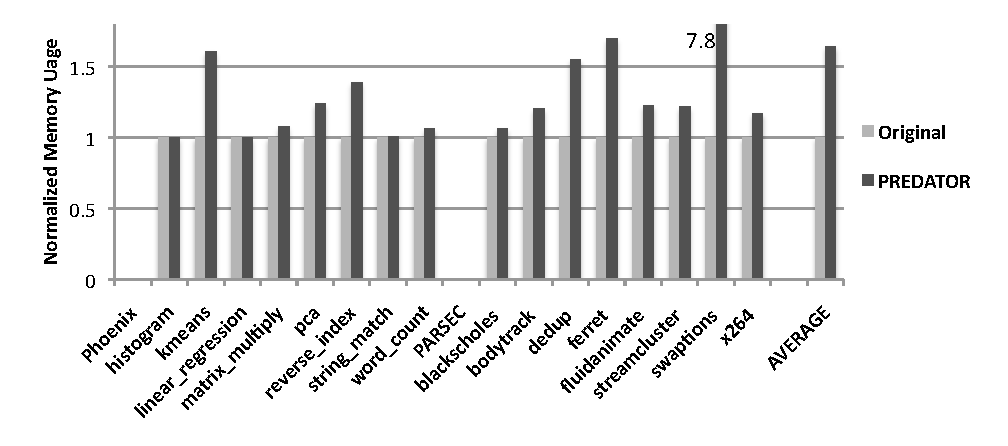
\includegraphics[width=5in]{fig/memusage}
\end{center}
%\includegraphics{fig/potential.pdf}
\caption{Memory usage overhead}
\label{fig:memusage}
\end{figure*}




\section{Discussion}
\label{sec:discussion}

This section analyzes some key limitations of \dthreads{} that
restrict its ability to run certain programs, limit the extent of
determinism it can guarantee, or potentially affect performance.

%\dthreads{} is a fully deterministic multithreaded system, which ensures a deterministic order of 
%both synchronization operations and all memory accesses. The most close
%work to us is CoreDet~\cite{Bergan:2010:CCR:1736020.1736029}.


\textbf{Unsupported programs: }
\dthreads{} currently does not support programs with ad hoc
synchronization that avoids the \pthreads{} library, such as those
that use atomic operations implemented in assembly.  However, the
upcoming C++0X standard includes a library interface for atomic
operations~\cite[pp. 1107--1128]{c++0xstandarddraft}, and a future
version of \dthreads{} could correctly implement these by intercepting
these library calls and treating them as synchronization points. While
ad hoc synchronization is a common practice, it is also a notorious
source of bugs; Xiong et al.\ show that 22--67\% of the uses of ad hoc
synchronization lead to bugs or severe performance
issues~\cite{ad-hoc-considered-harmful}.

\dthreads{} also currently does not write-share the stack
across threads, so that updates made by a thread to a stack variable
would not be reflected back to the parent, which could cause a program
to fail. Passing stack variables to a thread for modification is
extremely error-prone and generally deprecated, making this a rare
coding practice.

\textbf{External determinism: }
While \dthreads{} provides internal non-determinism, it does not
guarantee determinism when a program's behavior depends on external
sources of non-determinism, such as system time or I/O
events. Incorporation of \dthreads{} in the dOS framework, an OS
proposal that enforces system-level determinism, would provide full
deterministic execution, although this remains future
work~\cite{deterministic-process-groups}.

\textbf{Runtime performance: }
Section~\ref{sec:evaluation} shows that \dthreads{} can provide high
performance for a number of applications; in fact, for the majority of
the benchmarks examined, \dthreads{} matches or even exceeds the
performance of \pthreads{}. However, \dthreads{} does occasionally
degrade performance, sometimes substantially. The primary culprit is
the intensive use of locks (that is, when programs that acquire and
release locks at high frequency), which are much more expensive
in \dthreads{} than in \pthreads{}. The \texttt{ferret} benchmark from
the PARSEC benchmark suite exemplfies this behavior.

However, programmers using \dthreads{} could greatly reduce the use of
locks, and thus improve performance, by taking advantage
of \dthreads{}' strong isolation guarantee between threads.


%  Since Surprise locking inside libraries. Not a limitation \emph{per
%  se} but definitely an issue that could surprise programmers.

% Draft can be downloaded from http://www.open-std.org/jtc1/sc22/wg21/docs/papers/2010/n3126.pdf.
%Fine once they are library calls, as they are in gcc and in the upcoming C++0X standard (cite!), since then we can intercept them.

\textbf{Memory consumption: }
Finally, because \dthreads{} creates private, per-process copies of
modified pages between commits, it can increase a program's memory
footprint by the number of modified pages between synchronization
operations. This increased footprint does not seem to be a problem in
practice, both because the number of modified pages is generally far
smaller than the number of pages read, and because it is transitory:
all private pages are relinquished to the operating system
(via \munmap{}) at the end of every commit operation.

%Increased memory footprint (linear in the number of dirtied (modified) pages).




\section{Related Work}
\label{sec:relatedwork}

This section describes related work in false sharing detection, prevention, or both; no prior work predicts false sharing.

\subsection{False Sharing Detection}
Schindewolf et al.\ designed a tool based on the SIMICS functional simulator to report different kinds of cache usage information, such as cache misses and cache invalidations~\cite{falseshare:simulator}. Pluto relies on the Valgrind dynamic instrumentation framework to track the sequence of memory read and write events on different threads, and reports a worst-case estimation of possible false sharing~\cite{falseshare:binaryinstrumentation1}.
Similarly, Liu uses Pin to collect memory access information, and reports total cache miss information~\cite{falseshare:binaryinstrumentation2}.
These tools impose about $100-200\times$ performance overhead.

Zhao et al.\ present a tool based on the DynamoRIO framework to detect false sharing and other cache contention problems
for multithreading programs~\cite{qinzhaodetection}. 
It uses a shadow memory technique to maintain memory access history and detects cache invalidations based on the ownership of cache lines. However, it can only support at most $8$ threads. In addition, it cannot differentiate cold cache misses from actual false sharing problems.

Intel's performance tuning utility (PTU) uses Precise Event Based Sampling (PEBS) hardware support to detect false sharing problems~\cite{detect:ptu,detect:intel}.  PTU cannot distinguish true sharing from false sharing. In addition, PTU aggregates memory accesses without considering memory reuse and access interleavings, leading to numerous false positives. Sanath et al.\ designed a machine learning based approach to detect false sharing problems. They train their classifier on mini-programs and apply this classifier to general programs~\cite{mldetect}. Instead of instrumenting memory accesses, this tool relies on hardware performance counters to collect memory accesses events. This approach operates with extremely low overhead but ties false sharing detection to a specific hardware platform.

In addition to their individual disadvantages,
all approaches discussed above share a common shortcoming:  
they cannot pinpoint the exact location of false sharing in the source code, so programmers must manually examine the source code to identify problems.

Pesterev et al.\ present DProf, a tool that help programmers identify cache misses based on AMD's instruction-based sampling hardware~\cite{DProf}. DProf requires manual annotation to locate data types and object fields, and cannot detect false sharing when multiple objects reside on the same cache line.

\subsection{False Sharing Prevention}

Jeremiassen and Eggers use a compiler transformation to automatically adjust the memory layout of applications through padding and alignment~cite{falseshare:compile}. Chow et al.\ alter parallel loop scheduling in order to avoid false
sharing~\cite{falseshare:schedule}. These approaches only works for regular, array-based scientific code.

Berger et al.\ describe Hoard, a scalable memory allocator that can reduce the possibility of false sharing by making different threads use different heaps~\cite{Hoard}. Hoard cannot avoid false sharing problem in global variables or within a single heap object: the latter appears to be the primary source of false sharing problems.

\subsection{False Sharing Detection and Prevention}

\sheriff{} provides two tools to handle false sharing based on its ``threads-as-processes'' framework~\cite{sheriff}.
\Sheriff{}'s detection tool reports false sharing accurately and precisely with only $20\%$ performance overhead.
However, it can only detect write-write false sharing, and only works for programs that use the \pthreads{} library. It can also break programs that communicate across different threads with stack variables or \emph{ad hoc} synchronizations. These shortcomings limit \Sheriff{}'s usefulness for real-world applications.  
\Predator{} can detect all kinds of false sharing and imposes no limitations on the kind of applications it works on. 

\Sheriff{}'s prevention tool prevents false sharing altogether, eliminating the need for programmer intervention. However, in programs with many synchronization calls, the overhead imposed by \Sheriff{} could lead to performance degradation.

Plastic leverages the sub-page granularity memory remapping facility provided by the Xen hypervisor to detect and tolerate false sharing automatically~\cite{OSdetection}. However, the sub-page memory remapping mechanism is not currently supported by most existing operating systems, reducing its generality. In addition, Plastic cannot pinpoint the exact source of false sharing.  
In order to utilize Plastic's prevention tool, a program has to run on the Xen hypervisor, limiting the applicability of their prevention technique.


% eliminate global lock
% possibly adopting a page-ownership protocol as used by ...

\section{Conclusion}
This paper introduces \emph{evidence-based dynamic analysis}, a new
lightweight dynamic analysis technique. Evidence-based dynamic
analysis works for errors that can be forced to leave evidence of
their presence. These errors include key problems for C and C++
programs: buffer overflows, dangling-pointer errors, and memory
leaks. Evidence-based dynamic analysis is fast because it lets the
application run at full speed until an error is detected; execution is
then rolled back and replayed with instrumentation at the point where
the evidence was found, pinpointing the error. We
present \doubletake{}, the first evidence-based dynamic analysis
framework, and implement these analyses inside it. The resulting
analyses are the fastest versions to date, demonstrating the
effectiveness and efficiency of this new dynamic analysis approach.
\doubletake{} is available for download at \url{http://github.com/plasma-umass/DoubleTake}.



\section{Acknowledgements}
\begin{comment}
We want to thank Qiang Zeng, Dinghao Wu and Peng Liu for providing
their test cases used in their Cruiser paper.  We also thank Scott Kaplan for his
suggestions and comments in the development of \doubletake{}.
\end{comment}

{
\bibliographystyle{abbrv}
\bibliography{refs}
}

\end{document}
